


\section{Materials}
	Dust free cloths Super Polx 1200A \SI{23x23}{\cm} were bought from Berkshire.

	Patterned \gls{fto} substrates with sheet resistance of \SI{7}{\ohm\per\sq} (TEC7) on \SI{2.2}{\mm} thick and \SI{14.8x14.8}{\mm} wide Pilkington glass were bought from Xinyan Technology Ltd.

	Patterned \gls{ito} substrates with sheet resistance of \SI{15}{\ohm\per\sq} on \SI{1.1}{\mm} thick and \SI{15x15}{\mm} wide glass were bought from Xinyan Technology Ltd.

	All anhydrous and non-anhydrous solvents had a reagent grade purity; were purchased from Sigma-Aldrich and used without any additional treatment.

	Titanium(IV) isopropoxide (97~\%), acetylacetone, and \glsdesc{litfsi} (\gls{litfsi}) were bought from Sigma-Aldrich.

	\Gls{pedotpss} Clevios P VP.AI 4083 was bought from Heraeus.

	\ch{PbI2} (99~\%), \ch{PbBr2} (99.999~\%), \ch{CsI} (99.999~\%), \ch{PbCl2} (98~\%), anhydrous chlorobenzene, anhydrous \gls{dmf}, and anhydrous \gls{dmso} were bought form Sigma-Aldrich and kept in a nitrogen-filled glovebox.

	Methylamine in methanol (40~w/w\%, \SI{\approx9.8}{\Molar}) was bought from Tokyo Chemical Industry.

	\Gls{fai}, \gls{mabr} and \gls{mai} were either synthesised (described in \cpageref{methods-MAI}) or bought from GreatCell Solar (unknown purity).

	4-tert-butylpyridine and hydroiodic acid (57~w/w\% in water) were bought from Sigma-Aldrich and kept in a fridge (the colour of both these reagents change with ageing when kept out of the fridge, indicating degradation).

	\Gls{spiro} was bought from 1-Material and stored in a nitrogen-filled glovebox.

	\Gls{tae1}\index{TAE-1}, \gls{tae3}\index{TAE-3}, and \gls{tae4}\index{TAE-4} molecules (subject of the study in \cref{ch:tae}) were used as received from Dr.\ Inés García-Benito, Dr.\ Agustín Molina-Ontoria and Dr.\ Nazario Martín (IMDEA, Madrid).
	The synthesis of \gls{tae1}\index{TAE-1} has been described in \authoryear{Cabau2015a} and \authoryear{Choi2015b}.
	The synthesis of \gls{tae3}\index{TAE-3} and \gls{tae4}\index{TAE-4} has been described in \authoryear{Gelmetti2019}.

\section{Equipment}
	\epigraph{\textit{"Bring magnets with you\dots"}}

	\subsection{Equipments for Fabrication}

		\paragraph{Ultra-violet ozone cleaning system}
		Organic residuals removal was performed with a T10X10/OES UV/ozone cleaning system from UVOCS\@.
		Most common failure: insufficient gas extraction flow detected by differential pressure meter on the rear, it can be partially configured \textsl{via} a screw.
		It has been used for the treatment of \gls{fto} and \gls{ito} just prior to the deposition of titanium oxide precursors or \gls{pedotpss}.
		For the latter, this process improves the \gls{pedotpss} coverage increasing the support hydrophilicity.

		\paragraph{Spin coater in air atmosphere}
		Spin coating depositions in the clean room were performed with a Laurell WS-400BZ-6NPP-LITE spin coater.
		It has been used for deposition of titanium oxide precursors, \gls{pedotpss}, \gls{pcbm60}, and \gls{pcbm70}.

		\paragraph{Muffle oven}
		Calcination was performed with a muffle oven Hobersal HD-230 controlled with a Fuji Electric PXR-4.
		Most common failure: misuse of the controller by the users can cause unexpected excessive heating.
		It has been used for calcination of just-deposited dense titanium oxide thin films.

		\paragraph{Titanium hotplate}
		Calcination can be performed with a titanium hotplate Harry Gestigkeit PZ 28-3TD\@.
		Most common failures: controller failure and heating resistance breaks in a point, it can be unmounted and replaced.
		It has been used for calcination as an alternative to muffle oven.

		\paragraph{Glovebox}
		Perovskite deposition and precursors storage was done in a nitrogen-filled glovebox MBraun UNILab.

		\paragraph{Spin coater in inert atmosphere}
		Spin coating depositions in the nitrogen-filled glovebox were performed with a SPIN150 equipment (this model does not require a gas inlet, which would be troublesome in a glovebox) from SPS Europe where the transparent cap was removed from the lid for helping solvent vapours removal.
		For avoiding the accumulation of waste material, an aluminium foil was used for covering the deposition chamber and was replaced frequently.
		Most common failure: exhaustion of the supposedly \SI{20}{\year} lasting non-volatile SRAM (integrated circuit BattRam DS1230Y-85+ DIP28, a perfect example of planned obsolescence).
		It has been used for depositing the perovskite precursors and the \acr{htm} selective contacts.

		\paragraph{Precision hotplate}
		Annealing was performed with a highly homogeneous hotplate JP Selecta Plactronic.
		It has been used for annealing the just-deposited perovskite thin films.

		\paragraph{Thermal evaporator}
		High vacuum (\SI{1E-9}{\bar}) thermal depositions were performed with a MBraun vacuum deposition chamber connected with a scroll pump in series to a turbo pump.
		The deposition was controlled with an Inficom SQC310C unit (firmware version 6.44).
		The deposition rate was measured \textsl{via} two oscillating quartz sensors whose calibration tooling was performed yearly.
		The evaporation chamber was embedded in a MBraun MB200B glovebox module controlled by a MBraun MB20G.
		%inorganic and metallic materials%while the organic material deposition was controlled in a manual fashion with a CreaPhys temperature control unit CU~103
		It has been used for depositing the metallic electrodes, usually gold or silver.

	\subsection{Equipments for Materials Characterisation}

		\paragraph{Optical microscope}
		Optical microscopy images were acquired with a Leica S6 D microscope.
		It has been used for studying the homogeneity of the deposited thin films.

		\paragraph{UV--Vis--NIR spectrophotometer}
		Absorbance measurements were carried out on a Lambda 1050 PerkinElmer spectrophotometer equipped with a PhotoMultiplier Tube, \ch{InGaAs} and \ch{PbS} detectors system, double beam optics, double monochromator, \ch{D2} and \ch{W} light sources.
		It has been used for estimating the thickness of the deposited thin films.

		\paragraph{PhotoLuminescence spectrophotometer}
		Fluorescence measurements were carried out on a Fluorolog Horiba Jobin Yvon spectrofluorimeter equipped with photomultiplier detector, double monochromator, and Xenon light source.
		It has been used for the characterisation of molecules in solution.

		\paragraph{Time Resolved PhotoLuminescence spectrophotometer}
		PhotoLuminescence lifetime measurements were carried out on a Edinburgh Instruments LifeSpec-II based on the \gls{tcspc} technique, equipped with a PhotoMultiplier Tube detector, double subtractive monochromator and picosecond pulsed diode lasers source.
		It has been used for comparing the radiative recombination lifetime in perovskite thin films with or without selective contacts.

		\paragraph{X--ray diffractometer}
		\gls{xrd} measurements were made using a Bruker-AXS D8-Discover diffractometer equipped with parallel incident beam (Göbel mirror), vertical $\Theta$~-~$\Theta$ goniometer, XYZ motorised stage and with a GADDS (General Area Diffraction System).
		Samples were placed directly on the sample holder and the area of interest was selected with the aid of a video-laser focusing  system.
		An X-ray collimator system allows to analyse areas of \SI{500}{\um}.
		The X-ray diffractometer was operated at \SI{40}{\kV} and \SI{40}{\mA} to generate \ch{Cu} K$\alpha$ radiation.
		The GADDS detector was a HI-STAR (multiwire proportional counter of \SI{30x30}{\cm} with a \SI{1024x1024}{pixel}).
		We collected frames (2D \gls{xrd} patterns) covering \SIrange{15}{70}{\degree} $2\Theta$ from three different detector positions at a distance of \SI{15}{\cm} from the sample.
		The exposition time was \SI{300}{\s} per frame and it was chi-integrated to generate the conventional $2\Theta$ \textsl{versus} intensity diffractogram.
		Identification of the materials was achieved by comparison of the \gls{xrd} diffractogram with the ICDD data base (release 2007) using Diffracplus Evaluation software (Bruker 2007).
		It has been used for investigating the chemical composition of perovskite thin films after some months in contact with organic molecules.

		\paragraph{\Glsentryshort{esem} and \glsentryshort{esem}-\glsentryshort{edx} microscopes}
		Superficial and cross section \gls{esem} images were acquired at low voltage (beam accelerated with \SI{20}{\kV}) and high vacuum (\SI{1E-8}{\bar}) in a FEI Quanta 600 FEG microscope.
		The cut for cross section was performed mechanically: a small angle grinder (from Dremel) was used for furrowing a diagonal line on the substrate glass side (opposite to the \gls{fto}), then using two pliers the substrate was forced as if it was to bend the glass and opening further the furrow.
		It has been used for studying the homogeneity of the thin film coverage both from the top view and from the cross section.

		\paragraph{\Glsentryshort{afm} microscope}
		The \acrfull{ac-afm} imaging was done \textsl{via} \gls{afm} (Pico SPM II) and processed with WSxM software \cite{Horcas2007}.
		It has been used for confirming the coverage of the deposited thin films and for measuring their roughness.

		\paragraph{Profilometer}
		Thicknesses were measured furrowing layers with a hard object and measuring the elevation profile with an Ambios Tech.\ XP-1 profilometer.
		It has been used for measuring the thickness of the deposited layers thicker than \SI{100}{\nm}.

	\subsection{Equipments for Devices Electrical Characterisation}

		\paragraph{Devices holder}
		The devices holder is designed for holding 4 devices with 4 independent diodes each (the bottom electrode electrical contact is in common for all the diodes, the top electrodes contacts are independent) and consists in an airtight container topped with a quartz window.
		It was designed and fabricated by Ikerlan.
		The holder has at least one gold tip for each diode's electrode, the contact is ensured by springs pushing the tips towards the devices.
		A printed circuit board connects the gold tips to a coaxial connector \textsl{via} two rotatory selectors which allows to select the needed diode.
		It has been used for contacting the electrodes of the devices during all electrical measurements.

		\paragraph{Solar simulator}\label{solarsimulator}
		The illumination with accurate solar spectra was provided by a Sun 2000 solar simulator (\SI{150}{\W}) bought from ABET Technologies.
		The proper filters of the lamp were set to simulate the AM 1.5G solar spectrum.
		The light intensity at the measurement position was measured \textsl{via} the short circuit current of a small photodiode calibrated with a certified (NREL) silicon photodiode and regulated to \SI{1000}{\W\per\m\squared}.
		When needed, the light intensity was reduced using neutral filters.
		Most common failure: the power supply providing high voltage to the lamp.
		It has been used for illuminating the devices during current-voltage sweeps.

		\paragraph{Programmable digital multimeter}
		Currents and voltages were performed with a Tektronix Keithley 2400 (firmware revision C30) programmable digital source meter connected to a computer \textsl{via} a GPIB-USB-HS adapter from National Instruments, connected to the solar simulator for the shutter control \textsl{via} a RS-232 (Keithley side) to coaxial (solar simulator side), and connected to the device to measure \textsl{via} a coaxial (devices side) to 2 banana plugs (Keithley side).
		Most common failure: we observed sparks in the devices when connecting to the Keithley multimeter, so from our experience we recommend to manually set the Keithley in current measure mode with zero applied voltage, start the measure with the device not connected and finally connect the device.
		It has been used for registering the current-voltage sweeps.

		\paragraph{White \glsentryshort{led} illumination}
		White illumination at tunable intensity was provided \textsl{via} a white light \gls{led} ring with \gls{led} from LUXEON Lumileds and powered by a Aim-TTi PLH120-P power supply.
		It has been used for background illumination for \acrfull{ce}, \acrfull{tpv}, or \acrfull{tpc} measurement.

		\paragraph{Pulsed illumination}
		Perturbation illumination for photophysical characterisation was provided by a nanosecond PTI GL-3300 nitrogen laser.
		The pulse was triggered with a Aim-TTi TG330 analog function generator generating a square wave pulse.
		The pulse duration is around \SI{1.5}{\ns}.
		The wavelength was selected using the absorption and emission of a dissolved molecular dye.
		The pulse intensity was attenuated with a semi-transparent glass for ensuring the small perturbation regime.
		The equipment can output up to 20~pulses per second, but due to the oscilloscope internal memory speed we are limited to 1~pulse per second.
		It has been used for providing the illumination perturbation in \acrshort{tpv} characterisation.

		\paragraph{Oscilloscope}
		The voltage transients for photophysical characterisation were registered with a Yokogawa DLM2052 oscilloscope with an internal resistance of \SI{1}{\mega\ohm}, connected to the device holder \textsl{via} coaxial cable and to a computer \textsl{via} an USB2 port (the transfer speed could be better if an Ethernet connection were used).
		For each registered transient, \SI{12500}{points} were saved (the maximum record length for this oscilloscope is \SI{125}{Mpoints} and the maximum sampling rate is \SI{2.5}{Gpoints\per\s}).
		It has been used for measuring the voltage transients for the \acr{tpv}, \acr{tpc}, and \acr{ce} measurement.

		\paragraph{Switch for transient measurements}
		An equipment built in-house was used as a switch for opening and closing connections based on the input from a Aim-TTi TGP110 pulse generator.
		It has been used for simultaneously shutting down the white \gls{led} ring and short the devices during the \acr{ce} measurements.

		%FT-IR ATR
		%CycloVoltammetry CH instruments electrochemical workstation CHI660C
		%IPCE
		%red and blue LEDs
		%TAS
		%TEM
		%raman

\section{Synthesis, Handling and Purification}

	\subsection{\Glsentryshort{mai} Synthesis}\label{methods-MAI}

		%Reference in laboratory notebook: [ig15, ig18, ig31, ig83].

		\ch{CH3NH2 + HI\aq -> CH3NH3I\sld}

		The synthetic method was inspired by \cite{Im2011a}.
		In a \SI{500}{\ml} one-necked flask (over-dimensioned for easing the drying step) opened at air, \SI{14}{\ml} of a methylamine in methanol (\SI{40}{w/w\%}, \SI{\approx9.8}{\Molar}) were introduced.
		While stirring and cooling at \SI{0}{\celsius}, \SI{15}{\ml} of hydroiodic acid in water (\SI{57}{w/w\%}) was added drop-wise.
		The cooling was interrupted and the mixture was continuously stirred at room temperature.
		Then the vessel was left still overnight.
		The solution was evaporated in a vacuum-assisted rotatory evaporator at \SI{60}{\celsius}.
		The obtained white solid was scraped and transferred on a funnel with membrane filter (Sartorius, \gls{ptfe}).
		It was washed with diethyl ether and the diethyl ether discarded.
		The solid was dissolved with ethanol, using as little volume as possible and vacuum was used for forcing the ethanol through the filter.
		The solid was recrystallised pouring abundant diethyl ether, then filtered, washed with diethyl ether and dried at vacuum overnight.

	\subsection{Lead Salts Handling}

		Lead iodide and bromide bottles have to be opened in a nitrogen-filled glovebox.
		The failure in keeping the lead containing precursors away from oxygen causes the formation of insoluble derivatives, likely lead oxide or metallic lead, which will have to be filtered away from the precursors solution.

	\subsection{Dense Titania Precursors Solution}\label{precursors_tio2}

		The precursor solution for the dense \ch{TiO2} layer was prepared adding drop-wise \SI{0.38}{\ml} of acetylacetone to \SI{0.65}{\ml} of \iupac{titanium(IV) isopropoxide} and diluted in \SI{5}{\ml} of ethanol.
		Beware that the titanium-acetylacetone reaction is strongly exothermic.
		The solution can be used just for a few days after preparation.
		Some hydrolysed product can be present in the solution, so it has to be filtered (\gls{ptfe}, \SI{0.2}{\um}) just before the usage.

		An alternative synthetic route has been recently employed, starting from the stable and commercially available \iupac{titanium diisopropoxide bis(acetylacetonate)} as a convenient alternative: \SI{220}{\ul} of \ch{Ti(i-PrO)2(acac)2} in isopropanol (\SI{75}{w/w\%}, \SI{0.45}{\mmol}) were diluted adding \SI{1.28}{\ml} of isopropanol and filtered (\gls{ptfe}, \SI{0.2}{\um}) just before the usage.

	\subsection{\Glsentryshort{mapicl} Perovskite Precursors Solution}\label{precursors_mapicl}

		%The solution was prepared in the laboratory.
		In a vial, \SI{400}{\mg} of \gls{mai} (\SI{2.52}{\mmol}) and \SI{230}{\mg} of \ch{PbCl2} (\SI{98}{\%}, \SI{0.81}{\mmol}) were weighted.
		Then \SI{1}{\ml} of anhydrous \gls{dmf} was added and the solution was stirred at \SI{65}{\celsius} for \SI{1.5}{\hour}.
		The solution was not filtered and was used the same day of preparation.

	\subsection{\Glsentryshort{csfamapbibr} Perovskite Precursors Solution}\label{precursors_csfamapbibr}

		In a nitrogen-filled glovebox, \SI{507}{\mg} of \ch{PbI2} (\SI{99}{\%}, \SI{1.1}{\mmol}), \SI{73.4}{\mg} of \ch{PbBr2} (\SI{99.999}{\%}, \SI{0.200}{\mmol}), \SI{172}{\mg} of \gls{fai} (\SI{1.00}{\mmol}) and \SI{22.4}{\mg} of \gls{mabr} (\SI{0.200}{\mmol}) were weighted and mixed in a \SI{5}{\ml} vial.
		For reducing the effect of static charging on the weighting process in the glovebox, a stainless steel weighing boat was specifically fabricated.
		The mixed solid precursors can show some darkening due to the formation of perovskite in a solid-solid reaction (also known as mechanosynthesis \cite{Prochowicz2018}), nevertheless this solid mixture can be stored in the glovebox for weeks.

		The day of the deposition, \SI{0.2}{\ml} of anhydrous \gls{dmso} and \SI{0.8}{\ml} of anhydrous \gls{dmf} were added to the solid mixture of precursors.
		The solution was vigorously stirred at \gls{rt} for \SI{1}{\hour}.
		Heating or storing the solution for days has been observed to result in a yellow perovskite layer when deposited and annealed, so some kind of detrimental transformation is evident to happen in the solution, hindering its storage for long time.
		Finally \SI{42}{\ul} of	a \SI{1.5}{\Molar} \ch{CsI} solution in \gls{dmso} (\SI{63}{\umol}) were added to the previous solution.
		The solution was filtered (\gls{ptfe}, \SI{0.2}{\um}) just before its usage.
		The resulting stoichiometry is \ch{Cs_{0.06}FAMA_{0.2}Pb_{1.3}I_{3.2}Br_{0.6}}.

	\subsection{\Glsentryshort{spiro} and Other \glsentryshort{htm} Solutions}

		\paragraph{Additives mother solution}
		A solvent with additives mix was prepared adding \SI{197}{\umol} of 4-tert-butylpyridine (\SI{28.8}{\ul}) to \SI{1}{\ml} of anhydrous chlorobenzene, then \SI{32}{\umol} of \glsdesc{litfsi} (\gls{litfsi}, \SI{9.1}{\mg}) were added.
		The presence of 4-tert-butylpyridine enables the solubility of \gls{litfsi} in chlorobenzene (otherwise it would have to be dissolved in acetonitrile).

		\paragraph{\Glsentryshort{spiro}}
		\Glsdesc{spiro} solution was prepared dissolving \SI{59.0}{\umol} of \gls{spiro} (\SI{72.3}{\mg}) in \SI{1}{\ml} of the aforementioned solvent with additives mix.

		\paragraph{TAE-*}
		Other \acr{htm} solutions for bottom cathode cells were prepared dissolving either \SI{29.5}{\umol} of \glsdesc{tae1} (\gls{tae1}, \SI{36.6}{\mg}), \SI{19.7}{\umol} of \glsdesc{tae3} (\gls{tae3}, \SI{24.4}{\mg}), or \SI{9.83}{\umol} of \glsdesc{tae4} (\gls{tae4}, \SI{12.1}{\mg}) in \SI{1}{\ml} of solvent with additives further diluted with chlorobenzene in a 1:1, 1:2, 1:5 ratio respectively, in order to preserve the \acr{htm} to additives molar ratio of the \gls{spiro} solution (roughly \SI{3}{\eq} of 4-tert-butylpyridine and \SI{0.5}{eq} of \gls{litfsi}).
		The lower concentrations were used due to the lower solubility of these \acr{htm} as compared to \gls{spiro} one.

		\paragraph{Oxidation control}
		The \gls{spiro}, \gls{tae1}, \gls{tae3}, and \gls{tae4}\index{TAE-4} solutions did not include chemical oxidising agents and were prepared in a nitrogen-filled glovebox in order to have control over the oxygen oxidation degree of the molecules.

		\paragraph{\Glsentryshort{pedotpss}}
		\Glsdesc{pedotpss} (\gls{pedotpss}) was used as received from the commercial supplier.

		\FloatBarrier
		\newpage
\section{Perovskite Solar Cell Fabrication}
	\epigraph{\textit{\enquote{Making good devices is an art}}}

	The "top cathode" (or "illuminated anode", \cref{fig:top_cathode}) or "bottom cathode" (or "illuminated cathode", \cref{fig:bottom_cathode}) naming refers to the cell orientation during fabrication, so the "bottom" layer is the one closer to the glass substrate, as shown in \cref{fig:device_naming}.
	Both the top and the bottom cathode solar cells were fabricated following the scheme reported in \cref{fig:device_layout}.

	\begin{figure}
		\makebox[\textwidth][c]{
			\parbox{1.1\textwidth}{
				\centering
				\begin{subfigure}[t]{0.61\textwidth}
					\centering
					%					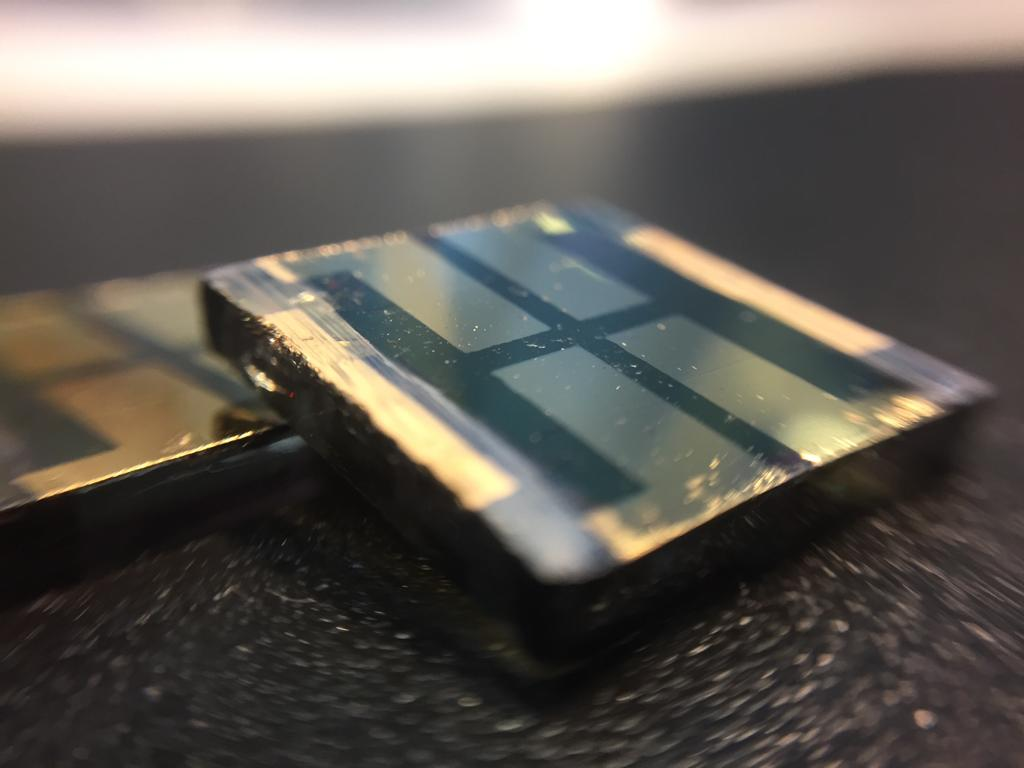
\includegraphics[width=0.4\textwidth]{device_picture/Perovskite_Palomares_ICIQ.jpeg}
					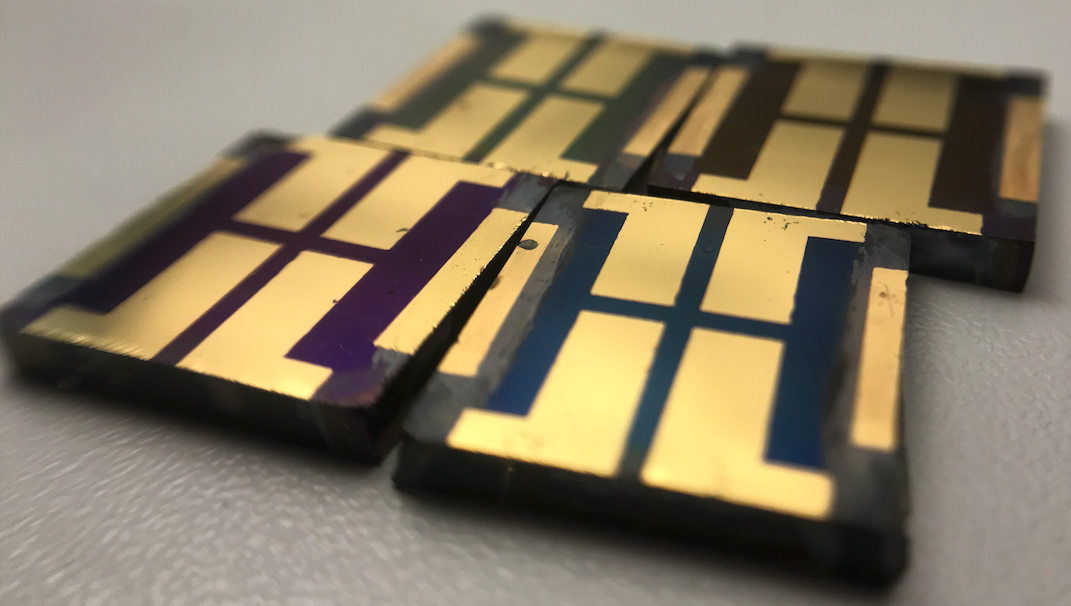
\includegraphics[width=0.8\textwidth]{device_picture/iciq_tae_news-crop.jpg}
					\subcaption{Bottom cathode perovskite solar cells}\label{fig:device_picture}
				\end{subfigure}
				\qquad
				\begin{subfigure}[t]{0.41\textwidth}
					\centering
					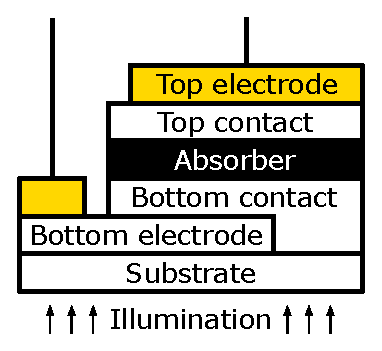
\includegraphics[width=0.9\textwidth]{bottom_top_naming/bottom_top_naming.pdf}
					\subcaption{Solar cell stack layers}\label{fig:device_naming}
				\end{subfigure}
				\bigskip

				\begin{subfigure}[t]{1.1\textwidth}
					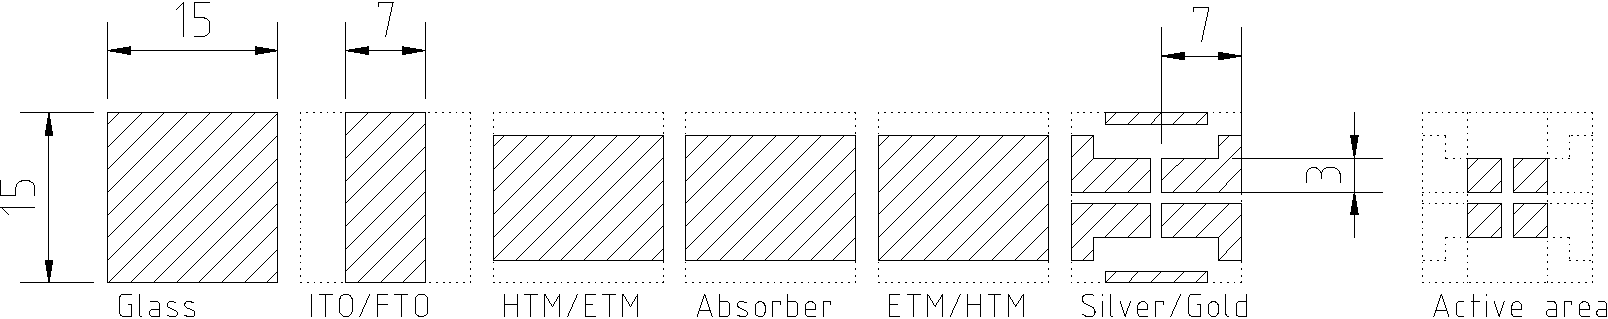
\includegraphics[width=1\textwidth]{device_layout/device_layout-crop.pdf}
					\subcaption{Schema of the layers}\label{fig:device_layout}
				\end{subfigure}

				\mycaption[Solar cells layers layout.]{
					In (\textbf{a}) a picture of typical bottom cathode perovskite solar cells is reported, each cell have a different \acr{htm} \cite{Gelmetti2019}.
					In (\textbf{b}) "top and bottom" naming is represented.
					The layers are named in the fabrication order, from the substrate up.
					The selective \acr{htm} and \acr{etm} contacts are named "contacts" just for brevity.
					The non-selective electrodes used for the electric connections are referenced as "electrodes".
					In (\textbf{c}) the shapes and dimensions of the utilised layers for top/bottom cathode solar cells are shown.
					From left to right: the glass substrate, the bottom transparent conducting oxide electrode, the bottom selective contact, the absorber, the top selective contact, the top metallic electrode.
					The active area is defined by the overlap of the \gls{ito}/\gls{fto} and the silver/gold layers, being \SI{9}{\square\mm}.}\label{fig:device}
			}
		}
	\end{figure}

	\FloatBarrier
	\subsection{Top Cathode Perovskite Solar Cells}\label{methods_top}

		\begin{SCfigure}
			\centering
			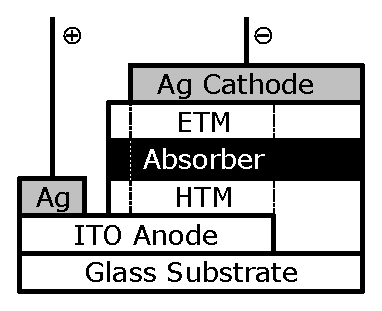
\includegraphics[width=0.4\textwidth]{bottom_top_cathode/top_cathode.pdf}
			\mycaption[Top cathode solar cell.]{The stack of a top cathode (or illuminated anode) solar cell.
				The shapes dimensions does not relate to real thicknesses and areas.
				The dashed lines indicate the active area.}\label{fig:top_cathode}
		\end{SCfigure}

		\paragraph{Anode and \glsentryshort{htm} substrate reparation}
		% based on ig77
		This process was performed in a ISO~7 clean room.
		\Gls{ito} coated substrates were cleaned in an ultrasound bath with acetone for \SI{15}{\min}, isopropanol for \SI{15}{\min} and rubbed with a dust-free cloth.
		Finally, an UV/ozone treatment was performed for \SI{20}{\min}.
		\Gls{pedotpss} was filtered on \gls{pes} membrane (\SI{0.22}{\um})
		and deposited \textsl{via} spin coating (static dispensing, \SI{110}{\ul}) with a first step where the speeds regulates the thickness of the layer and a second step for removing the residual liquid accumulated at the substrate corners.
		The conditions are reported in \cref{table:pedotpss_thickness} and the thicknesses were obtained \textsl{via} absorbance of light with wavelength \SI{2150}{\nm} calibrated to the a very thick layer measured with the profilometer.
		A rough relation between the thickness $d$ and the spinning speed $f$ (with \SI{1000}{\rpm\per\s} acceleration) was found as $d = \frac{1820}{\sqrt{f}}$.
		Substrates were dried at \SI{110}{\celsius} for \SI{20}{\min} and stored in a nitrogen-filled glovebox for avoiding moisture absorption.

		\begin{table}%[h]
			\caption{\Glsentrytext{pedotpss} deposition conditions and resulting thickness}\label{table:pedotpss_thickness}
			\begin{center}
				\begin{tabular}{c c c | c c c | c}
					\multicolumn{3}{c|}{\textbf{\nth{1} step}} & \multicolumn{3}{c|}{\textbf{\nth{2} step}} & \multirow{2}{*}{\textbf{thickness}}                                                                    \\
					acceleration                               & speed                                      & time                                & acceleration        & speed         & time        &              \\
					$[\si{\rpm\per\s}]$                        & $[\si{\rpm}]$                              & $[\si{\s}]$                         & $[\si{\rpm\per\s}]$ & $[\si{\rpm}]$ & $[\si{\s}]$ & $[\si{\nm}]$ \\[1mm]
					\hline
					\rule[0ex]{-4pt}{3ex}
					1000                                       & 1000                                       & 60                                  & 2000                & 2000          & 3           & 65           \\
					1000                                       & 1600                                       & 60                                  & 2000                & 2000          & 3           & 45           \\
					1000                                       & 4500                                       & 30                                  & 500                 & 3500          & 30          & 27           \\
				\end{tabular}
			\end{center}
		\end{table}

		\paragraph{\Glsentryshort{mapicl} perovskite one step fabrication}
		% ig71
		The deposition process was performed in a nitrogen-filled glovebox.
		The precursors solution (see \cpageref{precursors_mapicl}) was deposited \textsl{via} spin coating (\SI{80}{\ul}, static dispensing, loading time \SI{5}{\s}) with an acceleration of \SI{1000}{\rpm\per\s}, a speed of \SI{1900}{\s} for \SI{40}{\s}.
		The substrate was moved directly to a hotplate at \SI{100}{\celsius} and annealed for \SI{80}{\min}, resulting in a \SI{430}{\nm} thick perovskite layer.
		The film is colourless just after deposition, then it turns to brown, yellow and finally black on the hotplate.

		\FloatBarrier
		\paragraph{\Glsentryshort{mapi} perovskite two step fabrication}
		% based on ig79
		This process was performed in a nitrogen-filled glovebox.
		A constant purge of glovebox atmosphere is needed during the whole deposition process.
		This reduces the \gls{dmf} and \gls{dmso} vapours concentration avoiding damages to the formed perovskite layer and the poisoning of the glovebox oxygen removal catalysts.
		\SI{460}{\mg} of \ch{PbI2} were dissolved in \SI{1}{\ml} of a 23:2~v/v blend of anhydrous \gls{dmf} and anhydrous \gls{dmso}.
		This solution was stirred at \SI{50}{\celsius} for \SI{1}{\hour}.
		\SI{50}{\mg} of \gls{mai} were dissolved in \SI{1}{\ml} of a 3:1~v/v blend of anhydrous isopropanol and ethanol.
		A \ch{PbI2} layer was deposited from the unfiltered solution \textsl{via} spin coating (static dispensing, \SI{80}{\ul}, loading time \SI{5}{\s}) with accelerations and speeds reported in \cref{table:mapi_thickness}.
		After \SI{60}{\s} from the start of the spin coating, the \gls{mai} solution (\SI{100}{\ul}) was dynamically dispensed on the centre of the spinning substrate with a \SI{100}{\ul} micropipette keeping it tilted and depositing an uninterrupted stream.
		The substrate was then moved directly from the spin coater to a hotplate at \SI{100}{\celsius} and annealed for \SI{15}{\min}.
		The thicknesses reported in \cref{table:mapi_thickness} were measured using a profilometer.

		\begin{table}%[h]
			\caption{\Glsentrytext{mapi} two step deposition: conditions for the \ch{PbI2} and \gls{mai} spin coating and resulting perovskite film thickness.}\label{table:mapi_thickness}
			\begin{center}
				\begin{tabular}{c c c | c}
					acceleration        & speed         & time        & thickness    \\
					$[\si{\rpm\per\s}]$ & $[\si{\rpm}]$ & $[\si{\s}]$ & $[\si{\nm}]$ \\[1mm]
					\hline
					\rule[0ex]{-4pt}{3ex}
					2000                & 2000          & 90          & 440          \\
					4100                & 4100          & 90          & 320          \\
					8000                & 7500          & 90          & 230          \\
				\end{tabular}
			\end{center}
		\end{table}


		\paragraph{\Glsentryshort{etm} and cathode deposition}
		% based on ig75
		The solution was prepared in a ISO~7 clean room and the deposition process was performed in a nitrogen-filled glovebox.
		%(weighting fullerene derivatives in a glovebox would be difficult due to electrostatic phenomena)
		\SI{30}{\mg} of \gls{pcbm70} were dissolved in \SI{1}{\ml} of anhydrous chlorobenzene and stirred at \gls{rt} for \SI{1}{\hour}.
		This solution was filtered (\gls{ptfe}, \SI{0.2}{\um}) and deposited in a nitrogen-filled glovebox \textsl{via} spin coating (static dispensing, \SI{80}{\ul}, loading time \SI{5}{\s}) with accelerations and speeds reported in \cref{table:pcbm_thickness}.
		The thickness was estimated by absorbance with monochromatic illumination at \SI{378}{\nm} calibrating the highest point with a profilometer measurement.
		A rough relation between the thickness $d$ and the spin speed $f$ was found as $d = \frac{3930}{\sqrt{f}}$ when a concentration of \SI{30}{\mg\per\ml} in chlorobenzene was used.
		\Gls{ito} contact was cleaned on two edges using swabs slightly wet with chlorobenzene and then \gls{dmso} (the solvent vapours can damage the perovskite layer, so it is suggested to do this after \acr{htm} deposition which partially protects the underlying layer).
		\begin{table}%[h]
			\caption{\Glsentrytext{pcbm70} deposition conditions and resulting thickness, with a concentration of \SI{30}{\mg\per\ml}}\label{table:pcbm_thickness}
			\begin{center}
				\begin{tabular}{c c c | c}
					acceleration        & speed         & time        & thickness    \\
					$[\si{\rpm\per\s}]$ & $[\si{\rpm}]$ & $[\si{\s}]$ & $[\si{\nm}]$ \\[1mm]
					\hline
					\rule[0ex]{-4pt}{3ex}
					1100                & 1100          & 80          & 120          \\
					2000                & 2000          & 60          & 90           \\
					4000                & 4000          & 40          & 60           \\
					8000                & 7500          & 20          & 40           \\
				\end{tabular}
			\end{center}
		\end{table}
		Finally, \SI{120}{\nm} of silver were deposited by thermal evaporation in high vacuum (\SI{1E-9}{\bar}).
		This resulted in four independent \SI{0.09}{\cm\squared} diodes for each substrate.
		\label{methods_top_end}

		\FloatBarrier
	\subsection{Bottom Cathode Perovskite Solar Cells}\label{methods_bottom}

		\begin{SCfigure}
			\centering
			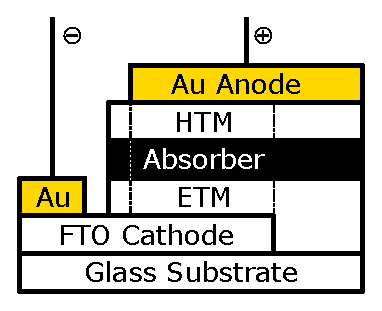
\includegraphics[width=0.4\textwidth]{bottom_top_cathode/bottom_cathode.pdf}
			\mycaption[Bottom cathode solar cell.]{The stack of a bottom cathode (or illuminated cathode) solar cell.
				The shapes dimensions does not relate to real thicknesses and areas.
				The dashed lines indicate the active area.}\label{fig:bottom_cathode}
		\end{SCfigure}

		\paragraph{Cathode and \glsentryshort{etm} substrate preparation}
		This process was performed in a ISO~7 clean room.
		Pre-patterned \SI{1.5 x 1.5}{\cm} \gls{fto} coated glasses were employed as substrate.
		The identification code was scratched with a diamond tip pencil.
		Initially the dust is removed with adhesive tape and rubbing with a dust free cloth.
		Then the substrates were cleaned with ultrasonication in water with Hellmanex soap, then in deionised water, and finally in isopropanol; dried rubbing with a dust free cloth and the organic residuals were removed with an UV/ozone treatment for \SI{20}{\min}.
		Dense (as opposed to mesoporous) \ch{TiO2} layer was deposited (static dispensing, \SI{80}{\ul}) from the solution described in \cpageref{precursors_tio2} by spin-coating at \SI{3000}{\rpm}, \SI{3000}{\rpm\per\s}, for \SI{60}{\s} (\SI{\approx 30}{\nm}) over the previously cleaned \gls{fto}.
		The substrates were placed in a glass Petri dish kept slightly open (this helps the removal of the burnt organic residuals and manages to reduce the entrance of dust) and inserted in a muffle oven.
		The sintering can also be performed placing the substrates on a titanium hotplate, but the amount of dust on the deposited layer is greater.
		Then the substrates were sintered at \SI{500}{\celsius} for \SI{30}{\minute} and cooled down slowly for not breaking the Petri dish.
		Subsequently the substrates were immersed in a filtered (\gls{pes}, \SI{0.22}{\um}) \SI{40}{\milli\Molar}
		\ch{TiCl4} solution in 9~\% \ch{HCl} in an oven at \SI{70}{\celsius} for \SI{20}{\min} (this process erode the titania layer, so it is important to not exceed in the duration), cleaned with water, with isopropanol and calcined as aforementioned at \SI{500}{\celsius} for \SI{30}{\min}.
		The usage of a thicker glass (\SI{2.2}{\mm}) as compared to the one used for top cathode cells (\SI{1.1}{\mm}) and the usage of \gls{fto} in place of \gls{ito} are needed for resisting the high temperature processing of the titania layer.
		Please note that \gls{fto} absorbs more in the infrared region than \gls{ito} and is more rough.

		%\paragraph{\Acr{mapi} Perovskite Two Step Fabrication}	
		% ig87

		\paragraph{\Glsentryshort{csfamapbibr} perovskite one step fabrication}

		This process was performed in a nitrogen-filled glovebox
		while constantly purging with a nitrogen flow for reducing the \gls{dmf} and \gls{dmso} vapours concentration.
		Perovskite precursor solution (see \cpageref{precursors_csfamapbibr}) was filtered (\SI{0.2}{\um}, \gls{ptfe})
		and deposited by spin-coating (\SI{80}{\ul}, static dispensing, first step \SI{1000}{\rpm}, \SI{1000}{\rpm\per\s}, \SI{10}{\s};
		second step \SI{6000}{\rpm}, \SI{1000}{\rpm\per\s}, \SI{20}{\s}; fast crystallisation was induced dynamically
		dispensing \SI{50}{\ul} of chlorobenzene on the spinning substrate \SI{5}{\s} before the end of the second
		step) obtaining a \SI{500}{\nm} thick perovskite layer.
		The substrates were immediately transferred from
		the spin coater to a hot plate and annealed at \SI{100}{\celsius} for \SI{60}{\minute}.
		After removing from the hotplate, the devices were stored in a glass Petri dish for protecting from dust deposition.
		It was left partially open to avoid accumulation of vapours from solvent residuals.

		\paragraph{\Glsentryshort{htm} and cathode deposition}
		The \acr{htm} solutions (\gls{spiro}, \gls{tae1}, \gls{tae3}, or \gls{tae4}) were filtered (\SI{0.2}{\um}, \gls{ptfe}) just before usage and deposited by spin-coating in a nitrogen-filled glovebox
		onto the perovskite layer (\SI{60}{\ul}, static dispensing, \gls{spiro} at \SI{4000}{\rpm}, \SI{4000}{\rpm\per\s},
		for \SI{30}{\s}; \gls{tae1}\index{TAE-1} and \gls{tae3}\index{TAE-3} at \SI{2000}{\rpm}, \SI{2000}{\rpm\per\s}, for \SI{30}{\s}; \gls{tae4}\index{TAE-4} at \SI{1000}{\rpm}, \SI{2000}{\rpm\per\s},
		for \SI{45}{\s}) and similar \acr{htm} thicknesses were obtained (\SI{\approx 100}{\nm}).
		\Gls{fto} contact was cleaned on two edges scratching away the \acr{htm} and perovskite materials; then the edges were further cleaned rubbing them with swabs slightly wet with \gls{dmso} (the solvent vapours can damage the perovskite layer).
		%, that's why this process is done after \acr{htm} deposition and just for what's remaining after mechanical scratching most of the material).
		Unless otherwise specified, in order to increase the
		oxidative doping of the \acr{htm} in a more or less controlled way, the devices were kept \SI{1}{\hour} in dark in a dry air chamber.
		Finally, \SI{80}{\nm} of gold was deposited by thermal evaporation in an ultra-high vacuum chamber
		(\SI{1e-9}{\bar}, MBraun) using a shadow mask leading to 4 diodes for substrate each with an active area of
		\SI{9}{\mm\squared}.
		\label{methods_bottom_end}


		\FloatBarrier
	\subsection{Handling and Preservation}

		\paragraph{Oxidative doping of \glsentryshort{htm}}
		In case of bottom cathode cells, the oxidation of the \acr{htm} has been proven to improve the \gls{pce}.
		The oxidation can be induced using dopants, for example FK 209 Co(III) TFSI salt\cite{Burschka2013} (this was not done in this thesis), or \textsl{via} oxygen exposure in dark.

		\paragraph{Degradation due to oxygen and illumination}\label{methods_degradation}
		As explained in \cpageref{intro_stability}, a synergic light and oxygen contribution on the perovskite layer degradation has been reported \cite{Senocrate2018a,Aristidou2017}.
		In \cref{fig:microscope_degradation} the degradation of a complete device exposed to continuous illumination for \SI{10}{\minute} and ambient air conditions is shown.
		An analogous device kept in air but without illumination did not show any degradation as observable \textsl{via} optical microscopy.
		The presence of mesoporous titania in the photographed solar cell helps the permeation of oxygen allowing the degradation to occur in every zone of the device.
		Interestingly the degradation is more prominent at metallic contacts' edges, one could speculate the reason being the electrical field being higher at smaller curvature metallic edges.
		It could also be that the ionic profile of perovskite when holes quasi Fermi level is pinned at gold workfunction makes perovskite more sensible to degradation, and this is more evident at edges due to oxygen diffusion being blocked by the gold layer.
		Even if storage in dark and dry air should not be damaging for perovskite solar cells, usually the long-term storage happens in a nitrogen-filled glovebox.


		%The oxygen can enter in direct contact with the perovskite layer due to permeability of the \gls{htm}; additionally, when a mesoporous \acr{etm} is used (e.g. titania) oxygen can diffuse rapidly through the partially infiltrated mesoporous structure. For this reason a cabinet has been modified adding of a constant dry air inlet. The gold contact was not enough for protecting the perovskite layer from degradation, as oxygen could penetrate through the mesoporous titania. 
		\begin{figure}%[!hbtp]%
			\makebox[\textwidth][c]{
				\parbox{1.1\textwidth}{
					\centering
					\begin{subfigure}[b]{0.3\textwidth}
						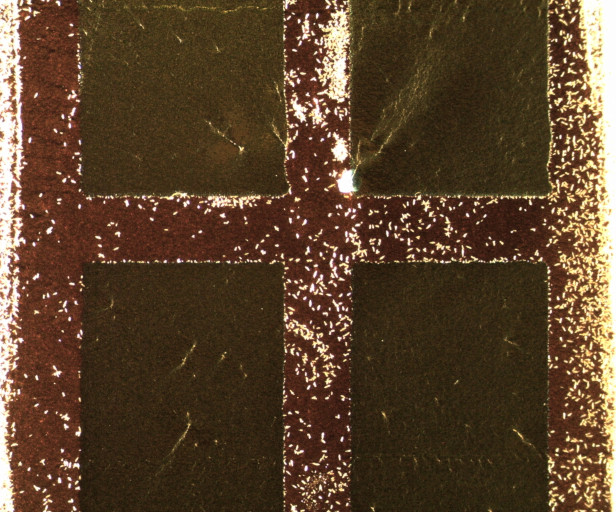
\includegraphics[width=1\textwidth]{microscope_degradation/ig93-1387-1-rescaled.jpg}
						\subcaption{Original, gold side.}\label{fig:microscope_degradation-start}
					\end{subfigure}
					\quad
					\begin{subfigure}[b]{0.3\textwidth}
						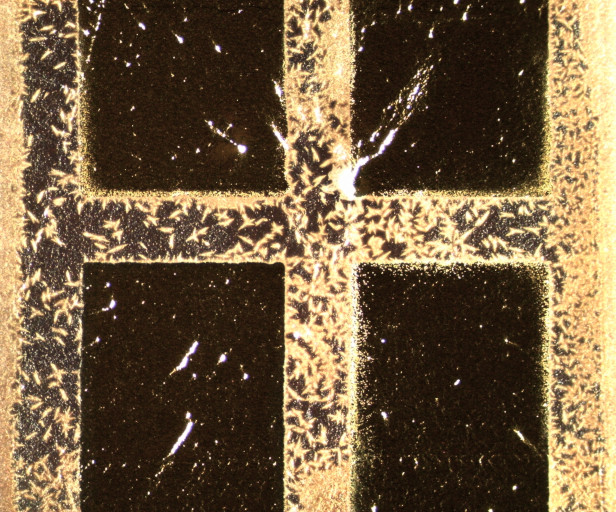
\includegraphics[width=1\textwidth]{microscope_degradation/ig93-1387-8-rescaled.jpg}
						\subcaption{\SI{10}{\minute}, gold side.}\label{fig:microscope_degradation-end_front}
					\end{subfigure}
					\quad
					%	\bigskip\newline
					%
					\begin{subfigure}[b]{0.3\textwidth}
						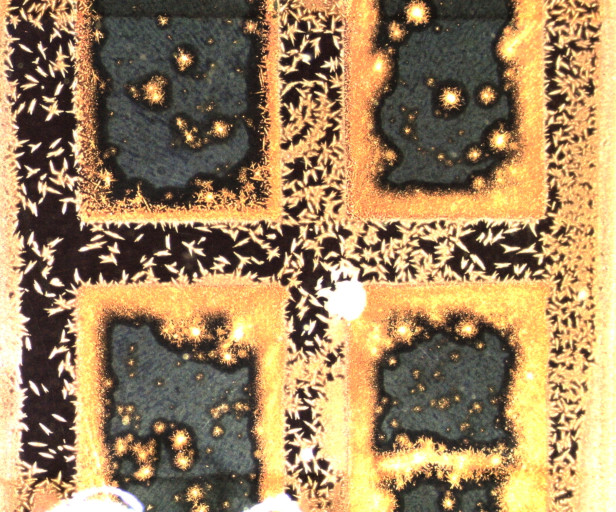
\includegraphics[width=1\textwidth]{microscope_degradation/ig93-1387-back-rescaled.jpg}
						\subcaption{\SI{10}{\minute}, glass side.}\label{fig:microscope_degradation-end_back}
					\end{subfigure}

					\mycaption[Degradation due to oxygen and illumination combination.]{A \gls{fto}\-/\ch{d-TiO2}\-/\ch{mp-TiO2}\-/\gls{csfamapbibr}\-/\gls{spiro}\-/\ch{Au} device upon \SI{10}{\minute} illumination in air.}\label{fig:microscope_degradation}
				}
			}
		\end{figure}


